\documentclass{article}

% if you need to pass options to natbib, use, e.g.:
% \PassOptionsToPackage{numbers, compress}{natbib}
% before loading nips_2018

% ready for submission
%\usepackage{nips_2018}

% to compile a preprint version, e.g., for submission to arXiv, add
% add the [preprint] option:
\usepackage[preprint]{nips_2018}

% to compile a camera-ready version, add the [final] option, e.g.:
% \usepackage[final]{nips_2018}

% to avoid loading the natbib package, add option nonatbib:
% \usepackage[nonatbib]{nips_2018}
% For citations

\usepackage[utf8]{inputenc} % allow utf-8 input
\usepackage[T1]{fontenc}    % use 8-bit T1 fonts
\usepackage{hyperref}       % hyperlinks
\usepackage{url}            % simple URL typesetting
\usepackage{booktabs}       % professional-quality tables
\usepackage{amsfonts}       % blackboard math symbols
\usepackage{nicefrac}       % compact symbols for 1/2, etc.
\usepackage{microtype}      % microtypography
\usepackage{graphicx}
\usepackage{placeins}

% For algorithms
\usepackage{algorithm}
\usepackage{algorithmic}
\usepackage{amsfonts}
\usepackage{amstext}
\usepackage{amssymb}
\usepackage{amsmath}

\title{Explanations for Multinomial Classifiers\\\vspace{10pt}\small{Tips and Tricks for Practitioners}}

% The \author macro works with any number of authors. There are two
% commands used to separate the names and addresses of multiple
% authors: \And and \AND.
%
% Using \And between authors leaves it to LaTeX to determine where to
% break the lines. Using \AND forces a line break at that point. So,
% if LaTeX puts 3 of 4 authors names on the first line, and the last
% on the second line, try using \AND instead of \And before the third
% author name.

% Authors in alphabetical order
\newcommand*\samethanks[1][\value{footnote}]{\footnotemark[#1]}
\author{
  Pramit Choudhary\thanks{H2O.ai}\\
  Los Angeles, CA\\
  \texttt{pramit.choudhary@h2o.ai}\\
  \And
  Navdeep Gill\samethanks\\
  Mountain View, CA\\
  \texttt{navdeep.gill@h2o.ai}\\ 
  \And
  Patrick Hall\thanks{H2O.ai and George Washington University}\\
  Washington, DC\\
  \texttt{patrick.hall@h2o.ai}}

\begin{document}

\maketitle

\begin{abstract}


\end{abstract}

\section{Introduction}

This short discussion bookends popular and practical texts on machine learning explanations by Chaudhary, Gill, Hall et al by specifically addressing the common and somewhat vexing problem of explaining the behavior and predictions of multinomial classifiers \cite{oreillymli}, \cite{art_and_sci}, \cite{oreillyskater}.  

%Difficulty of knowing if explanations are "right" -- this is why we chose simulated data.

%-------------------------------------------------------------------------------
\section{Notation} \label{sec:notation}
%-------------------------------------------------------------------------------

To facilitate technical descriptions of explanatory techniques, notation for input and output spaces, datasets, and models is defined.

\subsection{Spaces} 
 
	\begin{itemize}
		\item Input features come from the set $\mathcal{X}$ contained in a \textit{P}-dimensional input space,\\ $\mathcal{X} \subset \mathbb{R}^P$.  
		\item Known labels corresponding to instances of $\mathcal{X}$ come from the set $\mathcal{Y}$ contained in a \textit{C}-dimensional input space, $\mathcal{Y} \subset \mathbb{R}^C$.
		\item Learned output responses come from the set $\hat{\mathcal{Y}}$. For classification models the set $\hat{\mathcal{Y}}$ typically contains a column vector for each unique class in $\mathcal{Y}$. In this text, the space $\hat{\mathcal{Y}}$ is said to be contained in a $C'$-dimensional output space,  $\hat{\mathcal{Y}} \subset \mathbb{R}^{C'}$. 
%		\item The output responses come from a set $\mathcal{Y}$ contained in a $C$-dimensional output space (i.e. $\mathcal{Y} \subset \mathbb{R}^C$).
	\end{itemize}	
	
	\subsection{Datasets} 

	\begin{itemize}
		\item The input dataset $\mathbf{X}$ is composed of observed instances of the set $\mathcal{X}$ with a corresponding dataset of labels $\mathbf{Y}$, observed instances of the set $\mathcal{Y}$.
		\item Each $i$-th observation of $\mathbf{X}$ is denoted as $\mathbf{x}^{(i)} = $  
		$[x_0^{(i)}, x_1^{(i)}, \dots, x_{\textit{P}-1}^{(i)}]$, with corresponding $i$-th labels in $\mathbf{Y}, \mathbf{y}^{(i)} = [y_0^{(i)}, y_1^{(i)}, \dots, y_{\textit{C}-1}^{(i)}]$, and corresponding predictions in $\mathbf{\hat{Y}}, \mathbf{\hat{y}}^{(i)} =  [\hat{y}_0^{(i)}, \hat{y}_1^{(i)}, \dots, \hat{y}_{\textit{C'}-1}^{(i)}]$. % = [y_0^{(i)}, y_1^{(i)}, \dots, y_{\textit{C}-1}^{(i)}]$.
		\item $\mathbf{X}$ and $\mathbf{Y}$ consist of $N$ tuples of observations: $[(\mathbf{x}^{(0)},\mathbf{y}^{(0)}), (\mathbf{x}^{(1)},\mathbf{y}^{(1)}), \dots,$\\$(\mathbf{x}^{(N-1)},\mathbf{y}^{(N-1)})]$. %\\ $\mathbf{x}^{(i)} \in \mathcal{X}$, $\mathbf{y}^{(i)} \in \mathcal{Y}$.
		\item Each $j$-th input column vector of $\mathbf{X}$ is denoted as $X_j = [x_{j}^{(0)}, x_{j}^{(1)}, \dots, x_{j}^{(N-1)}]^T$.
	\end{itemize}	
	
	\subsection{Models}

	\begin{itemize}
		\item A type of machine learning model $g$, selected from a hypothesis set $\mathcal{H}$, is trained to represent an unknown signal-generating function $f$ observed as  $\mathbf{X}$ with labels $\mathbf{Y}$ using a training algorithm $\mathcal{A}$: 
		%\\ $\mathbf{X}, \mathbf{Y} \xrightarrow{\mathcal{A}} g$.
		\item $g$ generates learned output responses on the input dataset $g(\mathbf{X}) = \mathbf{\hat{Y}}$, and on the general input space $g(\mathcal{X}) = \hat{\mathcal{Y}}$.
		\item The model to be explained is denoted as $g$.
	\end{itemize}

%\section{Simulated Data Experiments}

\section{Global Analysis}

\subsection{Data}
Subsequent sections will use simulated data that empirically demonstrates the desired relationships between input feature importance and interactions in the input space $\mathbf{X}$, the label space $f(\mathbf{X}) = \mathbf{Y}$, a GBM model to be explained $g_{\text{GBM}}$, and a decision tree surrogate $h_{\text{tree}}$. Data with a known signal-generating function depending on four input features with interactions and with eight noise features is simulated such that: 

\begin{equation}
\label{eq:f}
f = \text{num} _1 * \text{num}_4 + |\text{num}_8| * \text{num}_9^2 + e
\end{equation}

\noindent$g_{\text{GBM}}$ is trained: $ \mathbf{X}, \mathbf{f(X)} \xrightarrow{\mathcal{A}} g_{\text{GBM}}$ such that $g_{\text{GBM}} \approx f$. Then $h_{\text{tree}}$ is extracted by $\mathbf{X}, g_{\text{GBM}}(\mathbf{X}) \xrightarrow{\mathcal{A}} h_{\text{tree}}$, such that $h_{\text{tree}}(\mathbf{X}) \approx g_{\text{GBM}}(\mathbf{X}) \approx f(\mathbf{X})$.

\subsection{Decision Tree Surrogate} \label{sec:surrogate_dt}

Given a learned function $g$, a set of learned output responses $g(\mathbf{X}) = \mathbf{\hat{Y}}$, and a tree splitting and pruning approach $\mathcal{A}$, a global -- or over all $\mathbf{X}$ -- surrogate decision tree $h_{\text{tree}}$ can be extracted such that $h_{\text{tree}}(\mathbf{X}) \approx g(\mathbf{X})$:

\begin{equation}
\mathbf{X}, g(\mathbf{X}) \xrightarrow{\mathcal{A}} h_{\text{tree}}
\end{equation}

\begin{figure}[htb]
	\begin{center}
		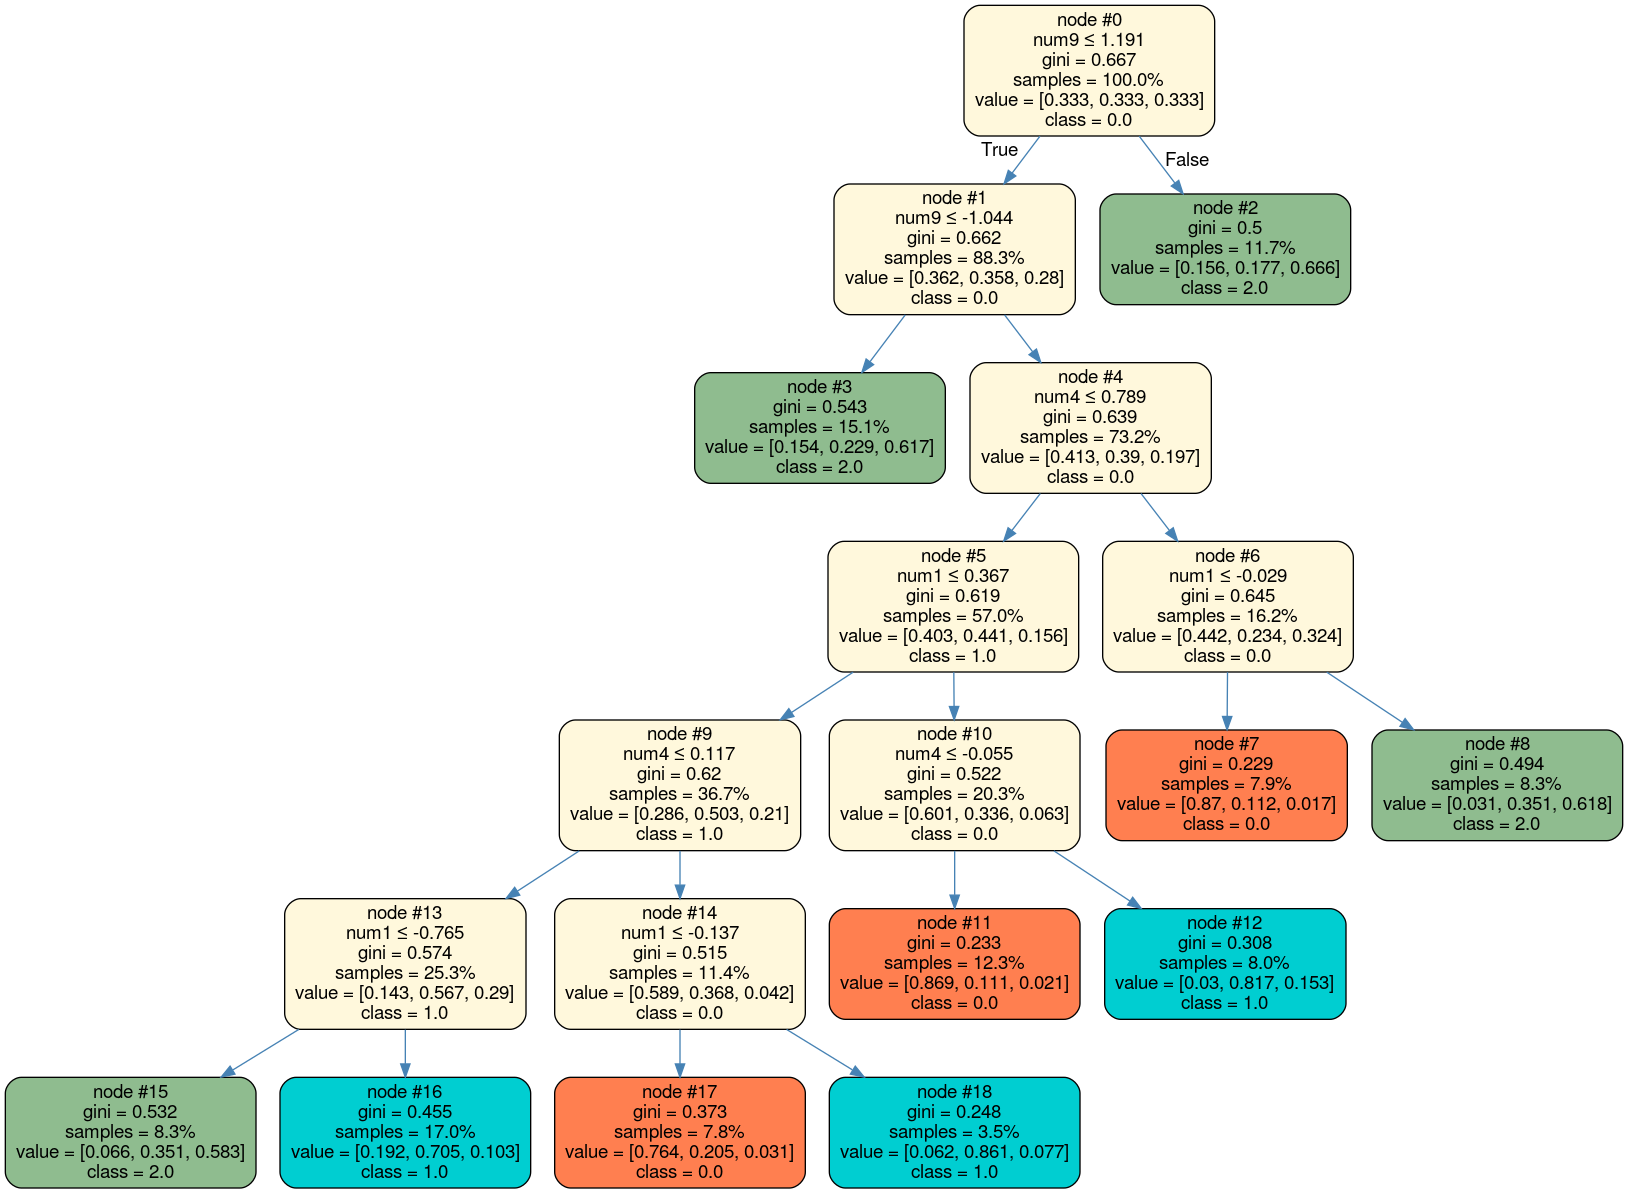
\includegraphics[height=200pt]{img/simple_tree_prepruned_simulated.png}
		\caption{}
		\label{fig:surrogate_dt}
	\end{center}
\end{figure}

Prescribed methods for training $h_{\text{tree}}$ do exist \cite{dt_surrogate1} \cite{dt_surrogate2}. In practice, straightforward cross-validation and pruning approaches are often sufficient. Moreover, comparing cross-validated training error to traditional training error can give an indication of the stability of the single decision tree $h_{\text{tree}}$.

Elegantly handles high cardinality targets.

\subsection{Decision Boundary Plots}

\begin{figure}[htb]
	\begin{center}
		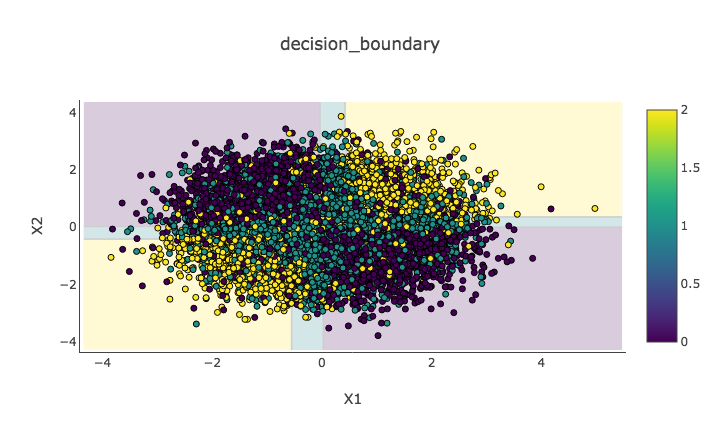
\includegraphics[height=120pt]{img/decision_boundary_simulated_num1_num4.png}
		\caption{}
		\label{fig:global_db}
	\end{center}
\end{figure}

What to do if very high cardinality in response, $\mathbf{Y}$:

\begin{itemize}

\item 2- or 3-D plot against most important variables
\item 2- or 3-D plot against sparse, interpretable extracted features: NMF, Sparse PCA

\end{itemize}

\subsection{Shapley Global Feature Importance}

Shapley explanations, including tree shap and even certain implementations of LIME, are a class of additive, consistent local feature contribution measures with long-standing theoretical support \cite{shapley}. Shapley explanations are the only possible locally accurate and consistent feature contribution values, meaning that Shapley explanation values for input features always sum to $g(\mathbf{x})$ and that Shapley explanation values can never decrease for some $x_j$ when $g$ is changed such that $x_j$ truly makes a stronger contribution to $g(\mathbf{x})$ \cite{shapley}. 

\begin{equation}
\label{eq:shap_additive}
\begin{aligned}
g(\mathbf{x}) = \phi_0 + \sum_{j=0}^{j=\mathcal{P} - 1} \phi_j \mathbf{z}_j
\end{aligned}
\end{equation}

\begin{equation}
\label{eq:shap_contrib}
\begin{aligned}
\phi_{j} = \sum_{S \subseteq \mathcal{P} \setminus \{j\}}\frac{|S|!(\mathcal{P} -|S| -1)!}{\mathcal{P}!}[g_x(S \cup \{j\}) - g_x(S)]
\end{aligned}
\end{equation}

Shapley values can be estimated in different ways. Tree shap is a specific implementation of Shapley explanations. It does not rely on surrogate models. Both tree shap and a related technique known as \textit{treeinterpreter} rely instead on traversing internal tree structures to estimate the impact of each $x_j$ for some $g(\mathbf{x})$ of interest \cite{tree_shap}, \cite{treeinterpreter}.

\begin{figure}[!htbp]
	\begin{center}
		\includegraphics[height=103pt]{img/shap_sim_horizontal_annotated.png}
		\caption{Shapley summary plot for known signal-generating function $f = \text{num} _1 * \text{num}_4 + |\text{num}_8| * \text{num}_9^2 + e$, and for learned GBM response function $g_{\text{GBM}}$ per response outcome.}
		\label{fig:global_feature_imp}
	\end{center}
\end{figure}
\FloatBarrier

\subsubsection{Recommendations}

What to do if very high cardinality in response, $\mathbf{Y}$:

\begin{itemize}

\item Examine top-K most frequent classes
\item Examine top-K most accurate and inaccurate classes
\item Examine classes with highest variance in sum(absolute(shap))

\end{itemize}

\subsection{Shapley Local Feature Importance}

\subsection{Partial Dependence and ICE}

Partial dependence (PD) plots are a widely-used method for describing the average predictions of a complex model $g$ across some partition of data $\mathbf{X}$ for some interesting input feature $X_j$ \cite{esl}. Individual conditional expectation (ICE) plots are a newer method that describes the local behavior of $g$ for a single instance $\mathbf{x} \in \mathcal{X}$. Partial dependence and ICE can be combined in the same plot to identify interactions modeled by $g$ and to create a holistic portrait of the predictions of a complex model for some $X_j$  \cite{ice_plots}.

\subsubsection{Description}
	
Following Friedman et al. a single feature $X_j \in \mathbf{X}$ and its complement set $\mathbf{X}_{(-j)} \in \mathbf{X}$ (where $X_j \cup \mathbf{X}_{(-j)} = \mathbf{X}$) is considered. $\text{PD}(X_j, g)$ for a given feature $X_j$ is estimated as the average output for a particular class outcome, $C'$, of the learned function $g(\mathbf{X})$ when all the components of $X_j$ are set to a constant $x \in \mathcal{X}$ and $\mathbf{X}_{(-j)}$ is left unchanged. $\text{ICE}(x_j, \mathbf{x}, g)$ for a given instance $\mathbf{x}$ and feature $x_j$ is estimated as the output for a particular class outcome, $C'$, for $g(\mathbf{x})$ when $x_j$ is set to a constant $x \in \mathcal{X}$ and all other features $\mathbf{x} \in \mathbf{X}_{(-j)}$ are left untouched. Partial dependence and ICE curves are usually plotted over some set of constants $x \in \mathcal{X}$. 

\begin{figure}[htb]
	\begin{center}
		\includegraphics[height=175pt]{img/pdp_ice_sim_annotated.png}
    \caption{Partial dependence and ICE curves per response outcome for previously defined known signal-generating function $f$,  learned GBM response function $g_{\text{GBM}}$, and important input feature $\text{num}_9$.}
    \label{fig:global_pdp_ice}
	\end{center}
\end{figure}

As in Section \ref{sec:surrogate_dt}, simulated data is used to highlight desirable characteristics of partial dependence and ICE plots. In Figure \ref{fig:global_pdp_ice} partial dependence and ICE at the minimum, maximum, and each decile of $g_{\text{GBM}}(\mathbf{X})$ are plotted per response outcome.

\subsubsection{Recommendations}

What to do if very high cardinality in response, $\mathbf{Y}$:

\begin{itemize}

\item Examine top-K most frequent classes
\item Examine top-K most accurate and inaccurate classes
\item Examine classes with highest variance in partial dependence
\item Examine classes with largest differences between partial dependence and ICE

\end{itemize}

\section{Supplementary Materials}

% Credit card use case, alternate figuree

UCI credit card dataset \cite{uci}.

\begin{center}
  \url{https://github.com/navdeep-G/interpretable-ml/tree/master/notebooks}
\end{center}

%\section{Credit Card Data Use Case}
%\subsection{Global Analysis}
%\subsubsection{Decision Tree Surrogate}
%\subsubsection{Decision Boundary Plots}
%\subsubsection{Shapley Global Feature Importance}
%\subsubsection{Partial Dependence and ICE}
%\subsection{Local Analysis: Local Shapley Feature Importance}

\section{Conclusion}

\section{NIPS Style examples}

\paragraph{Paragraphs}

There is also a \verb+\paragraph+ command available, which sets the
heading in bold, flush left, and inline with the text, with the
heading followed by 1\,em of space.

\subsection{Citations, figures, tables, references}
\label{others}

These instructions apply to everyone.

\subsection{Citations within the text}

The \verb+natbib+ package will be loaded for you by default.
Citations may be author/year or numeric, as long as you maintain
internal consistency.  As to the format of the references themselves,
any style is acceptable as long as it is used consistently.

The documentation for \verb+natbib+ may be found at
\begin{center}
  \url{http://mirrors.ctan.org/macros/latex/contrib/natbib/natnotes.pdf}
\end{center}
Of note is the command \verb+\citet+, which produces citations
appropriate for use in inline text.  For example,
\begin{verbatim}
   \citet{hasselmo} investigated\dots
\end{verbatim}
produces
\begin{quote}
  Hasselmo, et al.\ (1995) investigated\dots
\end{quote}

If you wish to load the \verb+natbib+ package with options, you may
add the following before loading the \verb+nips_2018+ package:
\begin{verbatim}
   \PassOptionsToPackage{options}{natbib}
\end{verbatim}

If \verb+natbib+ clashes with another package you load, you can add
the optional argument \verb+nonatbib+ when loading the style file:
\begin{verbatim}
   \usepackage[nonatbib]{nips_2018}
\end{verbatim}

As submission is double blind, refer to your own published work in the
third person. That is, use ``In the previous work of Jones et
al.\ [4],'' not ``In our previous work [4].'' If you cite your other
papers that are not widely available (e.g., a journal paper under
review), use anonymous author names in the citation, e.g., an author
of the form ``A.\ Anonymous.''

\paragraph{New preprint option for 2018}

If you wish to post a preprint of your work online, e.g., on arXiv,
using the NIPS style, please use the \verb+preprint+ option. This will
create a nonanonymized version of your work with the text
``Preprint. Work in progress.''  in the footer. This version may be
distributed as you see fit. Please \textbf{do not} use the
\verb+final+ option, which should \textbf{only} be used for papers
accepted to NIPS.

At submission time, please omit the \verb+final+ and \verb+preprint+
options. This will anonymize your submission and add line numbers to aid
review. Please do \emph{not} refer to these line numbers in your paper
as they will be removed during generation of camera-ready copies.

The file \verb+nips_2018.tex+ may be used as a ``shell'' for writing
your paper. All you have to do is replace the author, title, abstract,
and text of the paper with your own.

The formatting instructions contained in these style files are
summarized in Sections \ref{gen_inst}, \ref{headings}, and
\ref{others} below.

\subsection{Footnotes}

Footnotes should be used sparingly.  If you do require a footnote,
indicate footnotes with a number\footnote{Sample of the first
  footnote.} in the text. Place the footnotes at the bottom of the
page on which they appear.  Precede the footnote with a horizontal
rule of 2~inches (12~picas).

Note that footnotes are properly typeset \emph{after} punctuation
marks.\footnote{As in this example.}

\subsection{Figures}

\begin{figure}
  \centering
  \fbox{\rule[-.5cm]{0cm}{4cm} \rule[-.5cm]{4cm}{0cm}}
  \caption{Sample figure caption.}
\end{figure}

\subsection{Tables}

Place one line space before the table title, one line space after the
table title, and one line space after the table. The table title must
be lower case (except for first word and proper nouns); tables are
numbered consecutively.

Note that publication-quality tables \emph{do not contain vertical
  rules.} We strongly suggest the use of the \verb+booktabs+ package,
which allows for typesetting high-quality, professional tables:
\begin{center}
  \url{https://www.ctan.org/pkg/booktabs}
\end{center}
This package was used to typeset Table~\ref{sample-table}.

\begin{table}
  \caption{Sample table title}
  \label{sample-table}
  \centering
  \begin{tabular}{lll}
    \toprule
    \multicolumn{2}{c}{Part}                   \\
    \cmidrule(r){1-2}
    Name     & Description     & Size ($\mu$m) \\
    \midrule
    Dendrite & Input terminal  & $\sim$100     \\
    Axon     & Output terminal & $\sim$10      \\
    Soma     & Cell body       & up to $10^6$  \\
    \bottomrule
  \end{tabular}
\end{table}

The \verb+\bbold+ package almost always uses bitmap fonts.  You
  should use the equivalent AMS Fonts:
\begin{verbatim}
   \usepackage{amsfonts}
\end{verbatim}
followed by, e.g., \verb+\mathbb{R}+, \verb+\mathbb{N}+, or
\verb+\mathbb{C}+ for $\mathbb{R}$, $\mathbb{N}$ or $\mathbb{C}$.  You
can also use the following workaround for reals, natural and complex:
\begin{verbatim}
   \newcommand{\RR}{I\!\!R} %real numbers
   \newcommand{\Nat}{I\!\!N} %natural numbers
   \newcommand{\CC}{I\!\!\!\!C} %complex numbers
\end{verbatim}
Note that \verb+amsfonts+ is automatically loaded by the
\verb+amssymb+ package.

\subsubsection*{Acknowledgments}

Use unnumbered third level headings for the acknowledgments. All
acknowledgments go at the end of the paper. Do not include
acknowledgments in the anonymized submission, only in the final paper.

%-------------------------------------------------------------------------------
%\section{References}
%-------------------------------------------------------------------------------

\bibliographystyle{plain}
\bibliography{nips_multinomial_2018}
\end{document}